\documentclass[12pt, letterpaper]
{article}

% !TeX root = ../main.tex
\usepackage{a4wide}

\usepackage[utf8]{inputenc}

%\usepackage[ngerman]{babel}
\usepackage[english]{babel}

\usepackage[T1]{fontenc}
\usepackage{palatino}

\usepackage{graphicx}
\usepackage{caption}
\usepackage{url}
\usepackage{acronym}
\usepackage{tocloft}

\usepackage{mathpazo}
\usepackage{amsmath}
\usepackage{amsfonts}
\usepackage{adjustbox}

%\usepackage{subcaption}

\usepackage{hhline}
\usepackage{fancyhdr}
\usepackage{amssymb}
\usepackage{floatflt}
\usepackage{setspace}
\usepackage{float}
\usepackage{booktabs}
\usepackage{color}
\usepackage{listings}
\usepackage{array}
\usepackage{scrhack}
\usepackage{xcolor}
\usepackage{wrapfig}
\usepackage[hidelinks]{hyperref}
\usepackage{url}
\usepackage{lmodern}
\usepackage{multirow}
\usepackage{subfig}
\usepackage{cleveref}
\usepackage{lipsum}
\usepackage[bottom, hang]{footmisc}

% !TeX root = ../main.tex
%%%%%%%%%%%%%%%%%%%%%%%%%%%%%%%%%%%%%%%%%%%%%%%%%%%%%%%%%%%%%%%%%%%%%%%%
% Data about you and the Document%
%%%%%%%%%%%%%%%%%%%%%%%%%%%%%%%%%%%%%%%%%%%%%%%%%%%%%%%%%%%%%%%%%%%%%%%%

% % Main Title of Document:
\newcommand{\myMaintitle}{Comparing Articial Ingtelligence Algorithms by Solving Nonograms}

% % Sub Title of DocInput:
\newcommand{\mySubtitle}{My Subtitle}

% % Ihr Name:
\newcommand{\myName}{Dean Rossano}

% % Matrikelnummer:
% \newcommand{\myMatrikel}{MatNr: XXX}

% % Ihr Geburtsort:
\newcommand{\brith}{City}

% % Ihr Geburtsort:
\newcommand{\place}{City}

% % Ihr Abgabedatum:
\newcommand{\submission}{\today}

% % Ihr Abgabedatum:
\newcommand{\mycourse}{My Course}

% % Name des Betreuers/Erstprüfenden:
\newcommand{\fistSupervisor}{My Supervisor 1}
\newcommand{\secSupervisor}{My Supervisor 2}

% % In welchem Semester befinden Sie sich?
\newcommand{\mySemester}{Semester}

\title{\myMaintitle}

\author{\myName}

% !TeX root = ../main.tex
% % Linespread in main part
%\linespread{1.25}\selectfont

% Line spacing
%\onehalfspacing{}

%Path for Grafiken
\graphicspath{{fig/}}

%Stylerules
\widowpenalty10000 % Vermeidet einzelne Zeilen eines Absatzes zu Beginn einer Seite
\clubpenalty10000 % Vermeidet einzelne Zeilen eines Absatzes am Ende einer Seite
\addtocontents{toc}{\protect\sloppy}
\setcounter{tocdepth}{3}

\renewcommand{\headrulewidth}{.4mm} % header line width


% sloppy no right border override - bigger gabs
\sloppy

% % Set doc properties if 'hyperref' is present.
\hypersetup{pdftitle=\myMaintitle,pdfauthor=\myName,bookmarksopen=true}

% Source for picture captions
\newcommand{\source}[1]{\caption*{Source: {#1}} }

\newcommand{\code}[1]{\texttt{#1}}

\newcommand{\myparagraph}[1]{\paragraph{#1}\mbox{}\\}

\newcommand{\RM}[1]{\MakeUppercase{\romannumeral{} #1{}}}

\newcommand{\HRule}{\rule{\linewidth}{0.5mm}} % Defines a new command for horizontal


\definecolor{dkgreen}{rgb}{0,0.6,0}
\definecolor{gray}{rgb}{0.5,0.5,0.5}
\definecolor{mauve}{rgb}{0.58,0,0.82}

\lstset{ %
  language=Java,                  % the language of the code
  basicstyle=\footnotesize,       % the size of the fonts that are used for the code
  numbers=left,                   % where to put the line-numbers
  numberstyle=\tiny\color{gray},  % the style that is used for the line-numbers
  stepnumber=1,                   % the step between two line-numbers. If it's 1, each line
                                  % will be numbered
  numbersep=5pt,                  % how far the line-numbers are from the code
  backgroundcolor=\color{white},  % choose the background color. You must add \usepackage{color}
  showspaces=false,               % show spaces adding particular underscores
  showstringspaces=false,         % underline spaces within strings
  showtabs=false,                 % show tabs within strings adding particular underscores
  frame=single,                   % adds a frame around the code
  rulecolor=\color{black},        % if not set, the frame-color may be changed on line-breaks within not-black text (e.g. commens (green here))
  tabsize=4,                      % sets default tabsize to 2 spaces
  captionpos=b,                   % sets the caption-position to bottom
  breaklines=true,                % sets automatic line breaking
  breakatwhitespace=false,        % sets if automatic breaks should only happen at whitespace
  title=\lstname,                 % show the filename of files included with \lstinputlisting;
                                  % also try caption instead of title
  keywordstyle=\color{blue},          % keyword style
  commentstyle=\color{dkgreen},       % comment style
  stringstyle=\color{mauve}         % string literal style
}

%%%%%%%%%%%%%%%%%%%%%%%%%%%%%%%%%%%%%%%%%%%%%%%%%%%%%%%%%%%%%%%%%%%%%%%%%%%%%%%%%%%%%%%%%
%Examples
%%%%%%%%%%%%%%%%%%%%%%%%%%%%%%%%%%%%%%%%%%%%%%%%%%%%%%%%%%%%%%%%%%%%%%%%%%%%%%%%%%%%%%%%%
% \pdfmarkupcomment[markup=Squiggly,color=green]{with pdfcomment}{move to the front}.
% \pdfmarkupcomment[markup=StrikeOut,color=red]{stupid}{replace stupid with funny}
% \pdfmarkupcomment[markup=Highlight,color=yellow]{Of course, you can highlight complete sentences.}{Highlight}
% \pdfcomment[icon=Note,color=blue]{insert graphic!}


\NewDocumentCommand{\codeword}{v}{%
\texttt{\textcolor{blue}{#1}}%
}

% \pagestyle{plain}
\pagestyle{fancy}
\fancyhf{}
\fancyhfoffset[L]{1cm} % left extra length
\fancyhfoffset[R]{1cm} % right extra length
\rhead{\thepage}
\lhead{\nouppercase\leftmark}
\cfoot{\fancyplain{}{\thepage} }

\begin{document}
\nocite{*}

\pagenumbering{gobble}
% % !TeX root = ../main.tex
%%%%%%%%%%%%%%%%%%%%%%%%%%%%%%%%%%%%%%%%%
% Academic Title Page
% LaTeX Template
% Version 2.0 (17/7/17)
%
% This template was downloaded from:
% http://www.LaTeXTemplates.com
%
% Original author:
% WikiBooks (LaTeX - Title Creation) with modifications by:
% Vel (vel@latextemplates.com)
% hegerdes (hegerdes@uni-osnabrueck.de)
%
% License:
% CC BY-NC-SA 3.0 (http://creativecommons.org/licenses/by-nc-sa/3.0/)
%
% Instructions for using this template:
% This title page is capable of being compiled as is. This is not useful for
% including it in another document. To do this, you have two options:
%
% 1) Copy/paste everything between \begin{document} and \end{document}
% starting at \begin{titlepage} and paste this into another LaTeX file where you
% want your title page.
% OR
% 2) Remove everything outside the \begin{titlepage} and \end{titlepage}, rename
% this file and move it to the same directory as the LaTeX file you wish to add it to.
% Then add \input{./<new filename>.tex} to your LaTeX file where you want your
% title page.
%
%%%%%%%%%%%%%%%%%%%%%%%%%%%%%%%%%%%%%%%%%

%----------------------------------------------------------------------------------------
%	TITLE PAGE
%----------------------------------------------------------------------------------------
%Titelseite
\begin{titlepage}
	\centering
	\thispagestyle{empty}
	\vfill
	\HRule\\[0.4cm]
	\vspace{8mm}
	\huge{\textbf{{\fontfamily{ppl}\selectfont
	\myMaintitle}}}\\
	\HRule\\[0.4cm]
	\vspace{9mm}

		\begin{center}
			\large
			\textit{Author}\\
			\textsc{\myName}\\ % Your name
		\end{center}


	\vspace{5cm}
	\large{\today}
	\vfill
	\end{titlepage}
	\newpage

% \tableofcontents
% \newpage
\newcounter{lastroman}
\setcounter{lastroman}{\value{page}}
\pagenumbering{arabic}
\maketitle
\section{Problem Definition}
%talk about csps, ac3 and mrv
    This project will measure the efficiency of the CSP algorithm by measuring its performance at solving a kind of puzzle known as nonograms.  Nonograms are grid based puzzles in which the player must determine if the cells are to be filled in or left blank. Grids can be any rectangular shape but are typically found as squares (N x N) where N is a multiple of 5. Whether a cell is filled or not is determined by sequence of numbers aligned with the rows and columns of the grid. If a sequence contains a single number, the associated line will contain that number of filled squares in a row. If a sequence contains 2 or more numbers, that line contains an uninterrupted line of squares equal to each number, followed by at least one empty space between each number in the order that those numbers appear. For example, the first row of the below nonogram contains only a three, therefore the first row has three cells in a row filled in. The second line contains a one followed by a  three, therefore it gets one square filled in followed by a line of three.


\begin{figure}[H]
    \centering
    {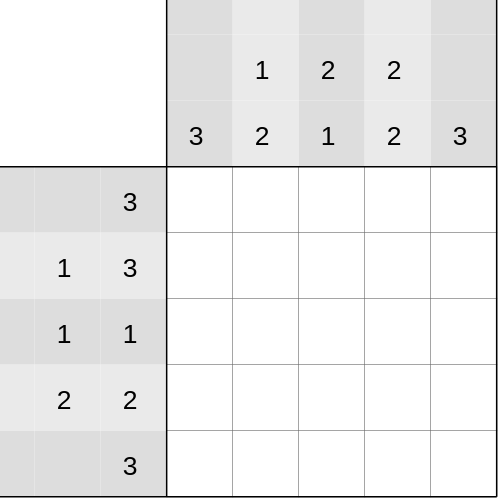
\includegraphics[width=0.4\linewidth]{fig/nonogram.png}}\hfill
    {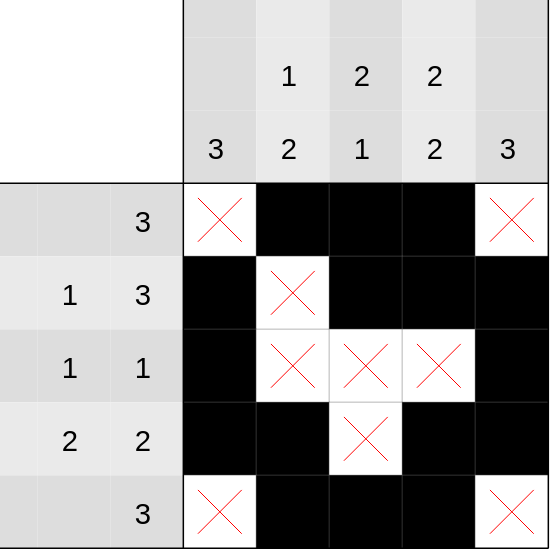
\includegraphics[width=0.4\linewidth]{fig/canvas.png}}
        \caption{An example nonogram and solution}
    \label{fig:example-nono}
\end{figure}

    Nonograms make for great problems to be solved by AI. The board and whether any square is determined to be filled, blank (denoted with an X), or unknown(left blank) is fully observable. As the solver is acting alone it will only have a single agent. The solver determines which squares are filled or not making them deterministic. Nonograms are sequential as squares being marked filled or blank will affect the possible outcome for other squares. Lastly as nonograms have well-defined rules they can be considered known environments. 
    
    An AI-based nonogram solver can be useful as a component for computer nonogram games. It can prvoide a player answers if they get stuck or be used to dynamically create puzzles iwth valid soltuions.

    \subsection{Constraint Satisfaction Problems}
    Nonograms will be structured as Constraint Satisfaction Problems (CSPs). CSPs are made up of three components: a set of variables, $X$, set of domains for each variable, $D$, and a set of contraints that are allowable combinations of values, $C$. Applying these principles to a nonogram: each row of the puzzle will be a variable. Based on the clues for a row, every possible combination of filled and unfilled cells will be found which will then compose the domain for that row. The constraints will be defined by the column clues; if each cell in a row creates a vaild column, that value satisfies the constraint.

    The AC-3 algorithm will be used to solve the CSPs generated by nonograms. In order to do this, the CSP will be structured as  driected graph known as a constraint graph. Nodes of the graph represent variables and arcs connect any two variables related by a constraint. AC-3 enforces arc-consistnecy in the graph; this means that each variable's domain satisifiess its constraints. A queue of all arcs in the CSP is created using tail, head notation. An arc is popped from the queue and checked if it is consistent. If it is the queue moves to the next arc, if not invalid values are removed from the tail. All arcs of constraints that point to the tail are then added to the queue. This repeats until either a domain is reduced to zero and it is determined that the CSP has no consistent solution, or no more arcs are in the queue and the CSP is solved.

    The Minimum Remaining Values(MRV) heuristic will be used to order the queue. This selects variables with the smallest domain first. It is also known as the 'fail-first' heuristic as it will select a variable with no legal values in its domain first and detect failure as immediately as it arrives. \cite{russell_artificial_2022}






\section{Previous Work}
    Manyam et al \cite{10863160} applied algorithms to solve Sudoku puzzles. As nonograms have well-defined rules like sudoku, similar studies can be conducted. Backtracking, Ant Colony Optimization(ACO) and Constraint Propagation Algorithms were implemented. They applied each of these algorithms to 9x9, 16x16 and 25 x 25 sudoku puzzles. A GUI for a sudoku game was created using the Pygame framework. The player can attempt to solve the puzzle themselves and when they get stuck, click on a button that will trigger an algorithm to solve the puzzle.

    The first algorithm that they implemented was Backtracking. The algorithm placed numbers in empty cells and upon reaching a conflict, backtracked by trying a different number in the cell. Branched that break constraints (the rules of sudoku) are pruned to increase efficiency. This is continued until either the puzzle is solved or every possibility is explored, and no solution can be found.

    ACO is implemented by simulating the behavior of ants. As cells are filled a "pheromone level" is assigned. The more likely to be valid that an entry is, the higher its pheromone level. Higher pheromone levels are more likely to be picked by future ants. Each cycle pheromone levels get updated and cells are filled accordingly until a solution is found, or all possibilities are exhausted.

    Lastly constraint propagation initialized the grid with possible values for empty cells and deletes impossible values to find cells that can be inferred with sudoku solving techniques. Invalid paths are eliminated, and the cycle repeats until the puzzle is solved.

    The results show that for girds sized 9x9 Constraint Propagation is the most efficient and for larger grids, ACO is the most efficient.

\section{Methodology}
%Expand on this
The performance of the AC-3 algorithm using the MRV heuristic to solve nonograms was be measured. The metrics to measure performance arwere execution time and accuracy. Accuracy was measured by comparing the results of the algorithm to the real solution of the nonograms.

The AC-3 algorithm was implemented in a command line Python program based on a Java prognam used for an assingment. Nonogram clues were supplied to the program in a CSV file. The first column of the csv represents clues for rows and the second column reperesents clues for columns. Clues are entered in the order they appear; top to bottom for rows, left to right for columns. Each individual number in a clue is separated with a space. Using figure \ref{fig:example-nono} as an example, a csv for its clues would be the following:
\begin{lstlisting}
3,3
1 3,1 2
1 1,2 1
2 2,2 2
3,3
\end{lstlisting}
For the accuracy comparison the solved nongram is also provided. It is formatted as a text file with \# representing filled cells and . representing blank cells. Each character has a leading space. Figure \ref{fig:example-nono}'s solution will be represented as shown:
\begin{lstlisting}
 . # # # .
 # . # # #
 # . . . #
 # # . # #
 . # # # .
\end{lstlisting}

The possible rows are calculated by taking the number of segments(each number in a clue) with the necessary blank spaces and calculating all possible combinations of positions those segments can take in a row. Pefore search began, AC-3 is run as pre-processing. It calls a revise function to remove any conflicting values from the tail.
Due to personal familiarity and the availability of the python-constraint \cite{pycon} library, the Python programming language will be used. The program will be a command line program that will solve nonograms. Nonograms will be supplied to the program via a CSV file where each column represents horizontal and vertical clues respectively, and each row represents clues for each row and column. These will be stored as arrays.
In modeling a nonogram as a Constraint Satisfaction Problem(CSP), the cells will be the variables, the domain will be the states of filled or empty and the constraints will be the clues for the puzzle. A method will be devised to determine if constraints are being violated. The time from the start of the CSP to it returning a result will be printed. The final nonogram will also be printed. This will be run for a 5x5, 10x10, 15x15 and 25x25 nonogram.

\section{Results}

\begin{lstlisting}
 # # # # . # # # # . . # # # # . # # # # . . # # #
 # # # # . # . . # . . # . . # . . # . . # . # # #
 # # . # # # . # # . # # . # # . # # . # # # . # #
 # # . . # . . . . . . . . . . . . . . . # . . # #
 # # . # # # # # # # # # # # # # # # . . . . . # #
 # # . . . # # # # # # # # # # # # # . . . . # # #
 # # . . # . # # # . . . . . . # # # . # . . . # #
 # # . # # . # . # . . . # . . . # . # # . . . # #
 # # . . # # # # . # . # . . # . # # # # . . . # #
 # # # . # # # . # . # . # . # # . . . . . . # # #
 # # # # # # . # # # . # . # . # # . . . # # # # #
 # # # # # . # # # . # . # . . . # # . # # # # # #
 # # . . # # # # . # # # # # # # # . # # # . . # #
 # . # # # . . . # # # . . # # . . # # # # . . . #
 # # . # # . # # # . . . . . # # # # # . . . . # #
 # # # . . . . . . . # # # . . . . . . . . . # # #
 # # . # . # . . # . # . # . # . # . . . . . . # #
 # . # # . . . # . . . # # # . # . # # . . . . . #
 # # . . . . # # # # # # # # # # # . . . . . . # #
 # # # # . . . . # . # # # # # . # . . . . . # # #
 . . # # . . . # # . . # # # . # # . . . . # # . .
 . # # # . # # . . # # # . # # # . . # # . # # # .
 # # # # # # # # . . # # # # # . . # # # # # # # #
 . # # # . . # # # . . . . . . . # # # . . # # # .
 # # . . # # # # # # # # # # # # # # # . . . # # .
\end{lstlisting}

\section{Conclusion}

% % Anhang
% \renewcommand{\thesubsection}{\Alph{subsection}}
% \pagenumbering{Roman}
% \setcounter{page}{\value{lastroman}}
% \section*{Appendix}
% \addcontentsline{toc}{section}{Appendix}

% %Abkürzungsverzeichnis
% % !TeX root = ../main.tex
\newcommand{\abbr}{Abbreviations}
\subsection*{Abbreviations}
\addcontentsline{toc}{subsection}{Abbreviations}

\begin{acronym}[1234567890]		%[längste Abkürzung]
\setlength{\itemsep}{-\parsep}	% sorgt dafür, dass das Verzeichnis kompakt dargestellt wird.

\acro{OS}[OS]{Operating System}


\end{acronym}
% \newpage

% %Code
% % !TeX root = ../main.tex
\subsection*{Code for you}
\addcontentsline{toc}{subsection}{Code for you}
\begin{lstlisting}[frame=single, caption={DemoCode},label=code::sttf]
    int main(){
        int i;

        // Line comment.
        puts("Hello world!");

        for (i = 0; i < N; i++){
            puts("LaTeX is also great for programmers!");
        }

        return 0;
    }
\end{lstlisting}
% \newpage
% \listoffigures
% \listoftables


%Bibliographie
\addcontentsline{toc}{section}{References}
\bibliographystyle{alpha}
\bibliography{bib/sources}

\end{document}